\section{Research Focus}

\begin{frame}{Fuel injector for Ammonia}

    \begin{columns}[c, onlytextwidth]

        \begin{column}{0.5\textwidth}

            Design a \textbf{direct Ammonia fuel injector compatible with current internal combustion engines}.

            \vspace{9pt}

            The key factors driving our design will be:

            \begin{itemize}
                \item Stable flame inside the combustion chamber
                \item Low-to-zero $\mathrm{NO_x}$ emissions
            \end{itemize}

        \end{column}

        \begin{column}{0.5\textwidth}

            \begin{figure}[H]
                \centering
                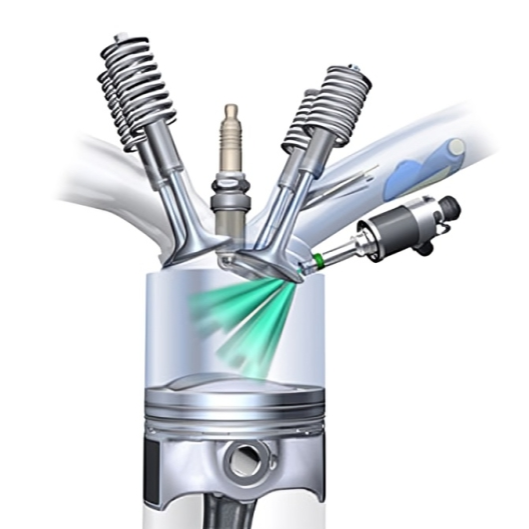
\includegraphics[width=0.9\textwidth]{img/injectors-in-ICE.png}
                \caption{Direct fuel injection in internal combustion engines}
            \end{figure}

        \end{column}

    \end{columns}

\end{frame}



\begin{frame}{Fuel injector for Ammonia}

    \begin{columns}[c, onlytextwidth]

        \begin{column}{0.4\textwidth}

            \begin{figure}[H]
                \centering
                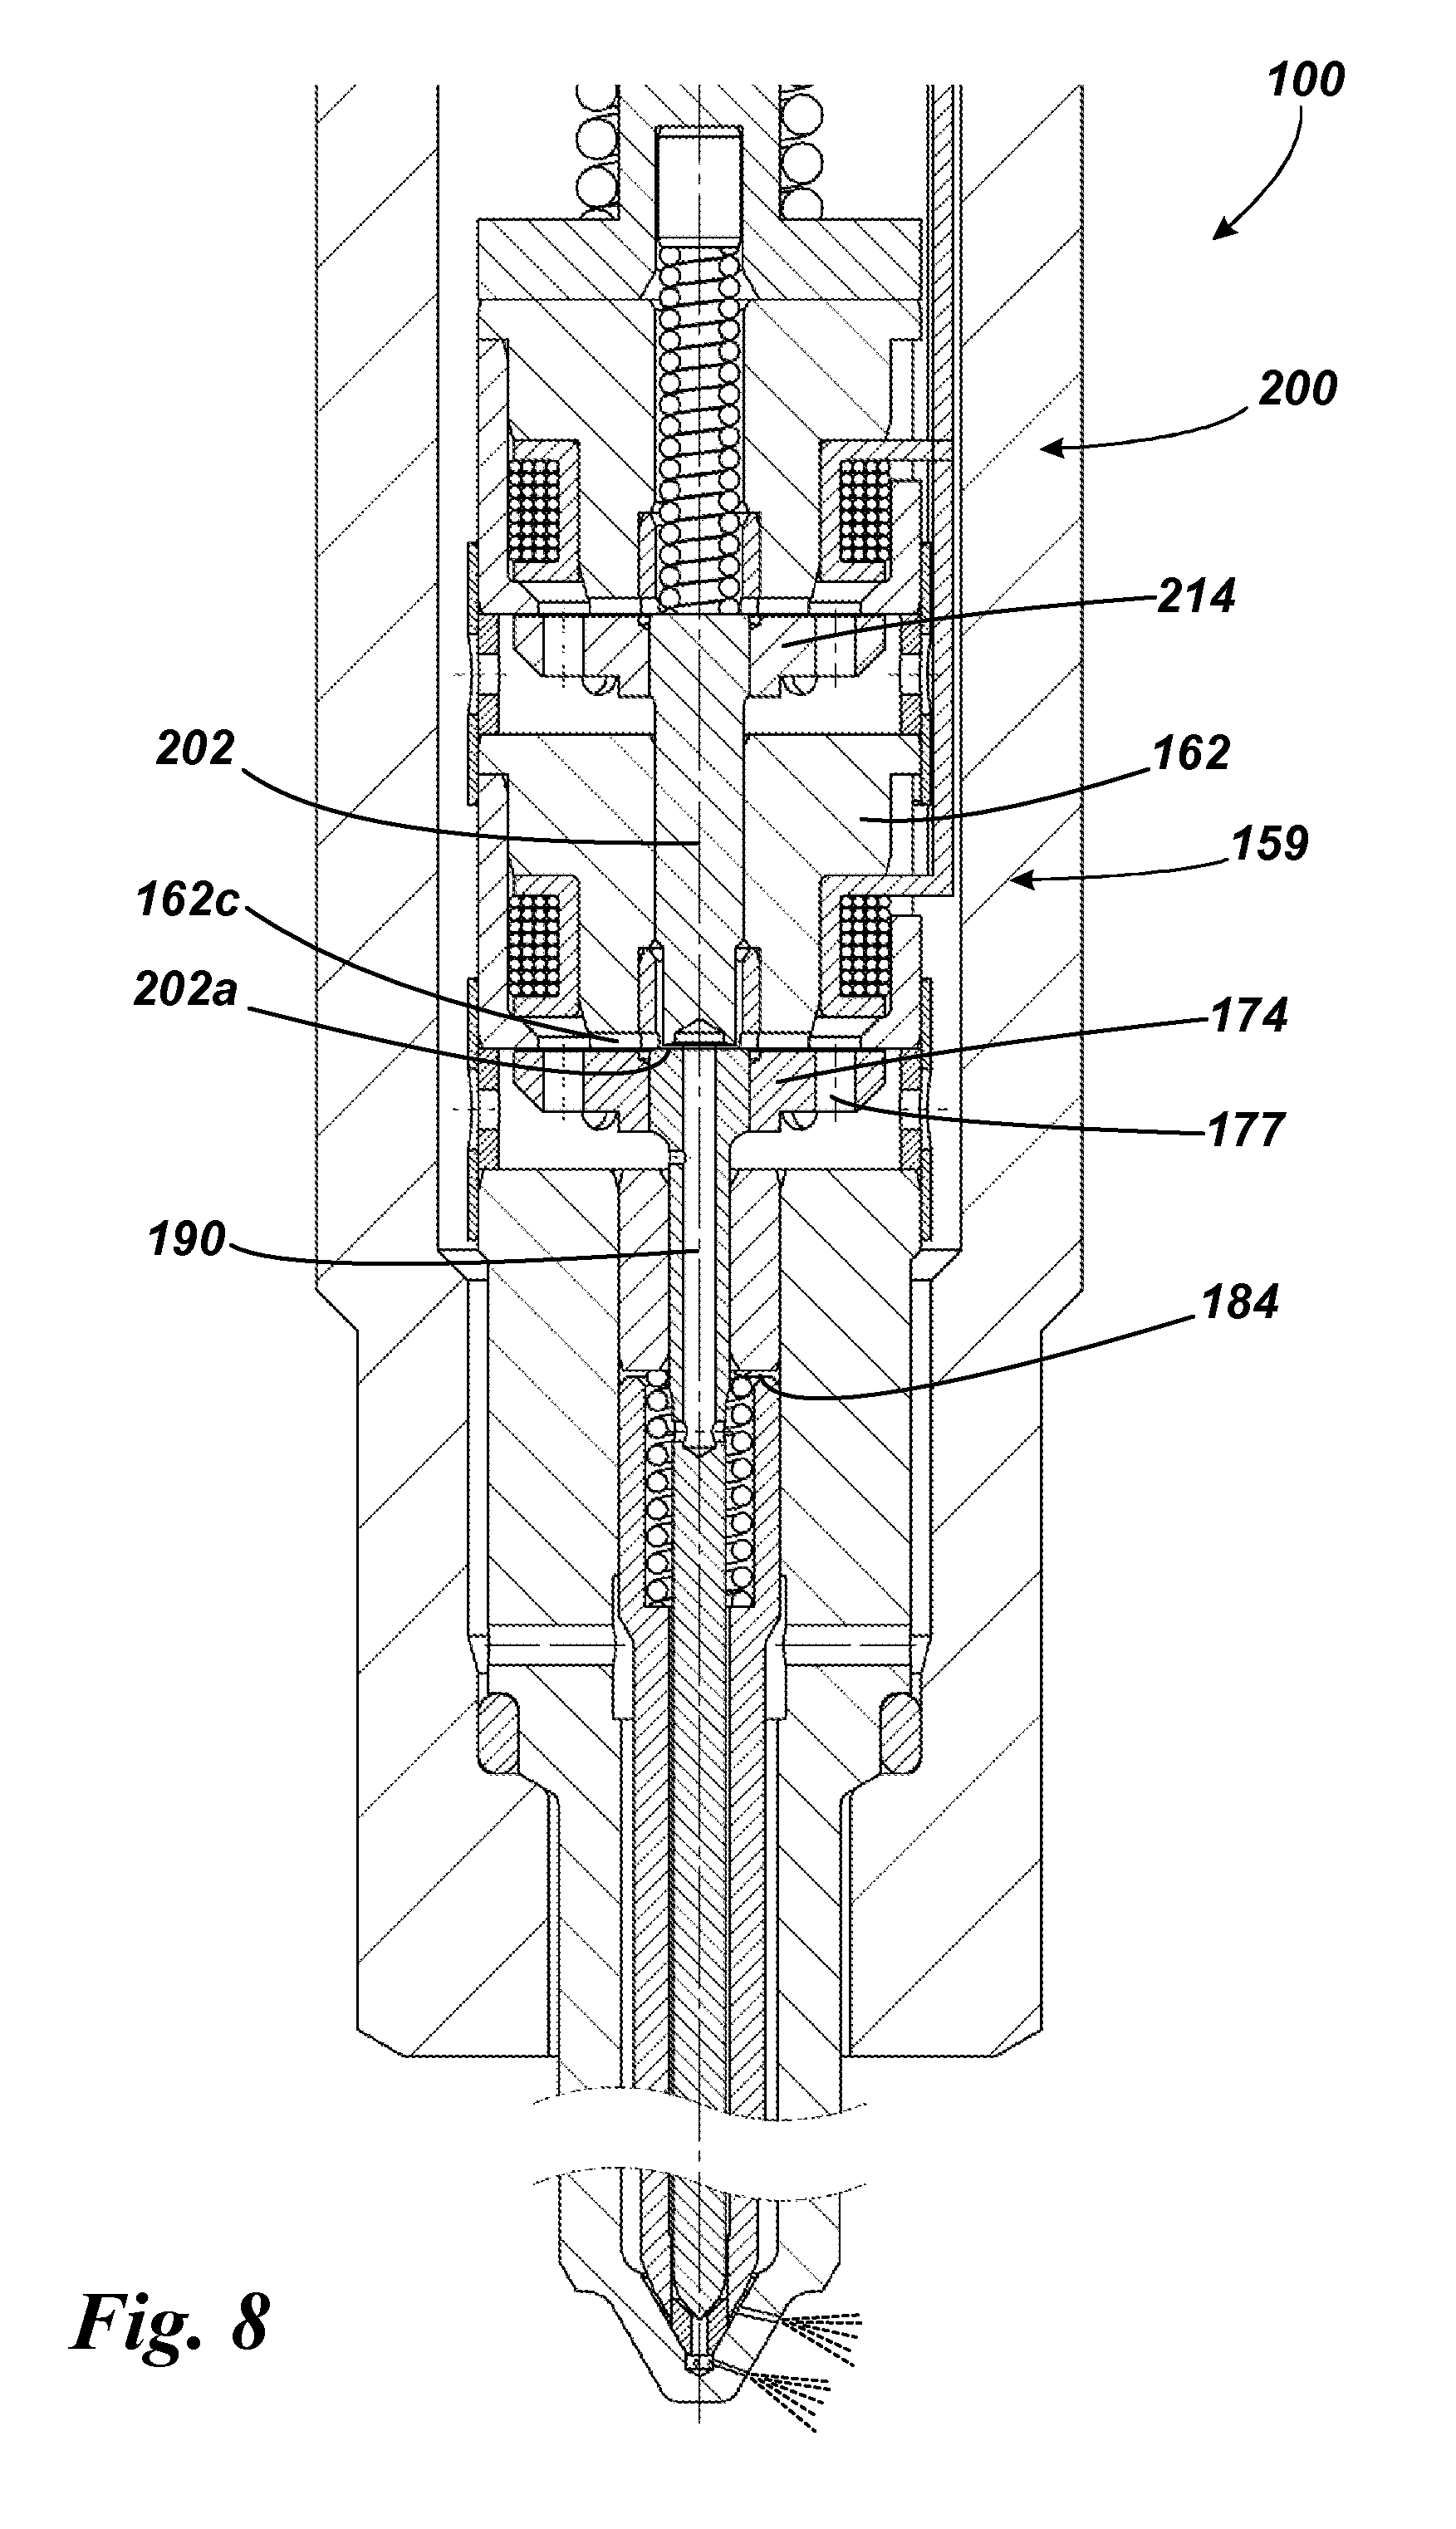
\includegraphics[width=0.8\textwidth]{img/injector-drawing.png}
                \caption{"Fuel injector" (US20120080011A1)}
            \end{figure}

        \end{column}

        \begin{column}{0.6\textwidth}

            The core focus will be on the \textbf{controllability of the atomization process}.

            \vspace{9pt}

            Given that, we also need to take into account the environmental working conditions:

            \begin{itemize}
                \item Temperatures (inlet, chamber, exhaust)
                \item Pressures (inlet, chamber, exhaust)
                \item Air-fuel ratio
                \item Injection timing
            \end{itemize}

        \end{column}

    \end{columns}

\end{frame}